\documentclass[tikz]{standalone}

% tikz
\usepackage{tikz, pgfplots}
% i wish external worked but idk it sucks
%\usetikzlibrary{external}
%\tikzexternalize[prefix=figures/]

% for function graph
\usetikzlibrary{positioning}
\usetikzlibrary{shapes.geometric}
\usetikzlibrary{positioning}
\usetikzlibrary{shapes.misc}
\tikzset{
dot/.style = {circle, fill=#1, minimum size=5pt,
              inner sep=0pt, outer sep=0pt},
dot/.default = black % size of the circle diameter
}
\tikzset{cross/.style={cross out, draw=black, minimum size=2*(#1-\pgflinewidth), inner sep=0pt, outer sep=0pt},
%default radius will be 1pt. 
cross/.default={1pt}}

 % for braces
\usetikzlibrary{decorations.pathreplacing}
% for hashing area
\usetikzlibrary{patterns}
% tableaux var, signe
% source https://www.sqlpac.com/fr/documents/latex-package-tkz-tab-tikz-tableaux-de-signes-et-de-variations-de-fonctions.html
\usepackage{tkz-tab}
\input{../colors}
\input{../letterfonts}


\tikzset{
	every node/.style = {font=\Large}
}

\tikzset{
	every axis/.style = {clip=true, grid style = {opacity=.5}}
}

\begin{document}
%
	% page 1
	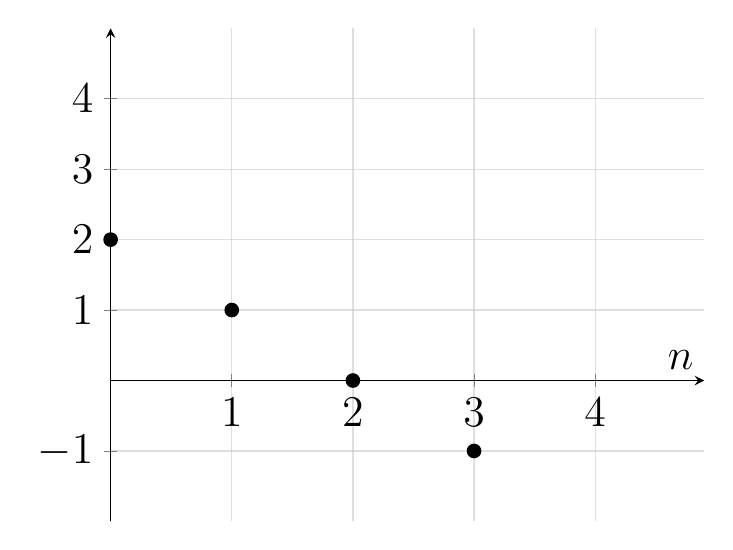
\begin{tikzpicture}[>=stealth, scale=1.1]
		\begin{axis}[xmin = 0, xmax=4.9, xtick={ 0,1,2, 3, 4,5}, ymin=-2, ymax=5, ytick={-1,0,1,2, 3,4}, axis x line=middle, axis y line=middle, axis line style=->, xlabel={$n$}, ylabel={}, grid=both]
			\addplot[black, thick, only marks, mark=*] coordinates {(0,2) (1,1) (2,0) (3,-1)};
		\end{axis}
	\end{tikzpicture}
	
	% page 2
	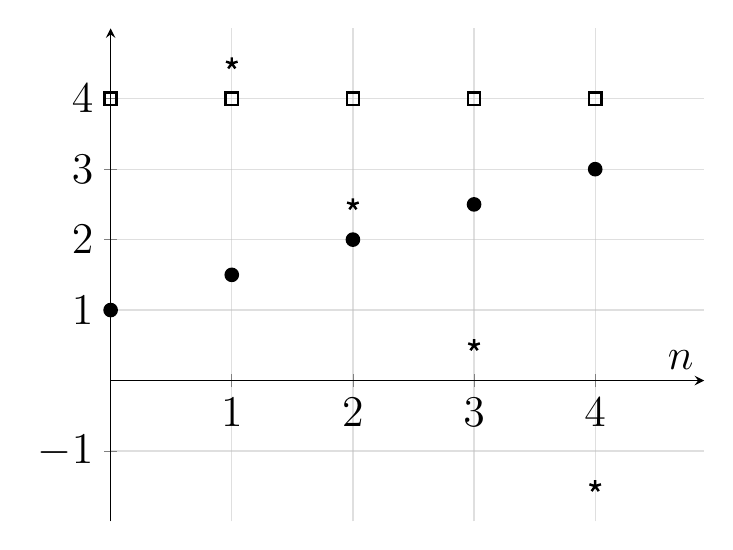
\begin{tikzpicture}[>=stealth, scale=1.1]
		\begin{axis}[xmin = 0, xmax=4.9, xtick={ 0,1,2, 3, 4,5}, ymin=-2, ymax=5, ytick={-1,0,1,2, 3,4}, axis x line=middle, axis y line=middle, axis line style=->, xlabel={$n$}, ylabel={}, grid=both]
			\addplot[black, thick, only marks, mark=*] coordinates {(0,1) (1,1.5) (2,2) (3,2.5) (4,3)};
			
			\addplot[black, thick, only marks, mark=star] coordinates {(1, 4.5) (2,2.5) (3,0.5) (4,-1.5)};
			
			\addplot[black, thick, only marks, mark=square] coordinates {(0,4) (1,4) (2,4) (3,4) (4,4)};
		\end{axis}
	\end{tikzpicture}
	
	% page 3
	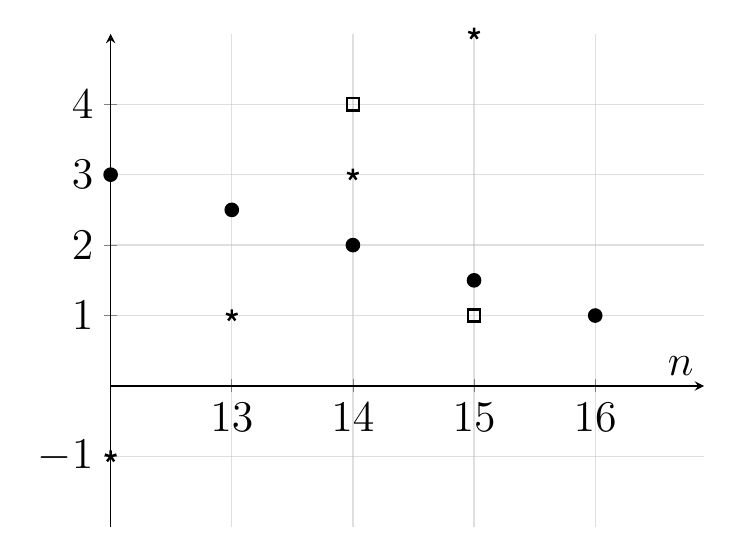
\begin{tikzpicture}[>=stealth, scale=1.1]
		\begin{axis}[xmin = 12, xmax=16.9, xtick={ 12,13,14,15, 16}, ymin=-2, ymax=5, ytick={-1,0,1,2, 3,4}, axis x line=middle, axis y line=middle, axis line style=->, xlabel={$n$}, ylabel={}, grid=both]
			\addplot[black, thick, only marks, mark=*] coordinates {(12,3) (13,2.5) (14,2) (15,1.5) (16,1)};
			
			\addplot[black, thick, only marks, mark=star] coordinates {(12,-1) (13,1) (14,3) (15,5)};
			
			\addplot[black, thick, only marks, mark=square] coordinates {(14,4) (15,1)};
		\end{axis}
	\end{tikzpicture}
		
	% page 4
	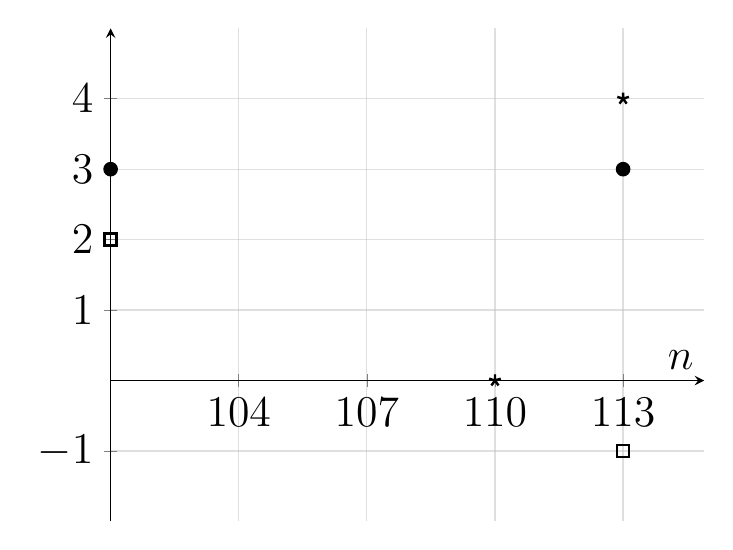
\begin{tikzpicture}[>=stealth, scale=1.1]
		\begin{axis}[xmin = 101, xmax=114.9, xtick={ 101,104,107,110,113}, ymin=-2, ymax=5, ytick={-1,0,1,2, 3,4}, axis x line=middle, axis y line=middle, axis line style=->, xlabel={$n$}, ylabel={}, grid=both]
			\addplot[black, thick, only marks, mark=*] coordinates {(101,3) (113,3)};
			
			\addplot[black, thick, only marks, mark=star] coordinates {(110,0) (113,4)};
			
			\addplot[black, thick, only marks, mark=square] coordinates {(101,2) (113,-1)};
		\end{axis}
	\end{tikzpicture}
%
\end{document}